\subsubsection{Resistor ixU}
\begin{figure} [H] 
    \centering
    \pgfplotstableset{
        columns/x/.style={
            column name={$U[V]$},
        },
        columns/y/.style={
            column name={$i[mA]$},
        },
        columns/ex/.style={
            column name={$\Delta U[V]$},
        },
        columns/ey/.style={
            column name={$\Delta i[mA]$},
        },
    }
    \pgfplotstableread{data/resistor.dat}\loadedtable
    \pgfplotstabletypeset{\loadedtable}
    \caption{Tabela de dados da corrente adquirida ao aumentar tensão em resistor}
    \label{fig:tableR}
\end{figure}

\begin{figure} [H] 
    \centering
    \begin{tikzpicture}
        \begin{axis}[
            width=10cm,
            xlabel={$U[V]$},
            ylabel={$i[A]$},
            xlabel style={below right},
            ylabel style={above left},
            ]
            \addplot [color=cyan, mark=o, smooth, ultra thick]
                plot [error bars/.cd, y dir = both, y explicit]
                table[x =x, y =y]{data/resistor.dat};
        \end{axis}
    \end{tikzpicture}
    \caption{Gráfico da corrente adquirida ao aumentar tensão em resistor}
    \label{fig:graphR}
\end{figure}

\subsubsection{Diodo ixU}
\begin{figure} [H] 
    \centering
    \pgfplotstableset{
        columns/x/.style={
            column name={$U[V]$},
        },
        columns/y/.style={
            column name={$i[mA]$},
        },
        columns/ex/.style={
            column name={$\Delta U[V]$},
        },
        columns/ey/.style={
            column name={$\Delta i[mA]$},
        },
    }
    \pgfplotstableread{data/diodo.dat}\loadedtable
    \pgfplotstabletypeset{\loadedtable}
    \caption{Gráfico da corrente adquirida ao aumentar tensão em diodo}
    \label{fig:tableD}
\end{figure}

\begin{figure} [H] 
    \centering
    \begin{tikzpicture}
        \begin{axis}[
            width=10cm,
            xmode=log,
            xlabel={$U[V]$},
            ylabel={$i[mA]$},
            xlabel style={below right},
            ylabel style={above left},
            ]
            \addplot [color=cyan, mark=o, smooth, ultra thick]
                plot [error bars/.cd, y dir = both, y explicit]
                table[x =x, y =y, x error=ex, y error=ey]{data/diodo.dat};
        \end{axis}
    \end{tikzpicture}
    \caption{Gráfico da corrente adquirida ao aumentar tensão em diodo}
    \label{fig:graphD}
\end{figure}


\subsubsection{Diodo RxU}
\begin{figure} [H] 
    \centering
    \pgfplotstableset{
        columns/x/.style={
            column name={$U[V]$},
        },
        columns/y/.style={
            column name={$R[\Omega]$},
        },
        columns/ex/.style={
            column name={$\Delta U[V]$},
        },
        columns/ey/.style={
            column name={$\Delta R[\Omega]$},
        },
    }
    \pgfplotstableread{data/diodo2.dat}\loadedtable
    \pgfplotstabletypeset{\loadedtable}
    \caption{Gráfico da resitência adquirida ao aumentar tensão em diodo}
    \label{fig:tableD2}
\end{figure}

\begin{figure} [H] 
    \centering
    \begin{tikzpicture}
        \begin{axis}[
            width=10cm,
            xmode=log,
            xlabel={$U[V]$},
            ylabel={$R[\Omega]$},
            xlabel style={below right},
            ylabel style={above left},
            ]
            \addplot [color=cyan, mark=o, smooth, ultra thick]
                plot [error bars/.cd, y dir = both, y explicit]
                table[x =x, y =y, x error=ex, y error=ey]{data/diodo2.dat};
        \end{axis}
    \end{tikzpicture}
    \caption{Gráfico da resistência adquirida ao aumentar tensão em diodo}
    \label{fig:graphD2}
\end{figure}


\begin{figure} [H] 
    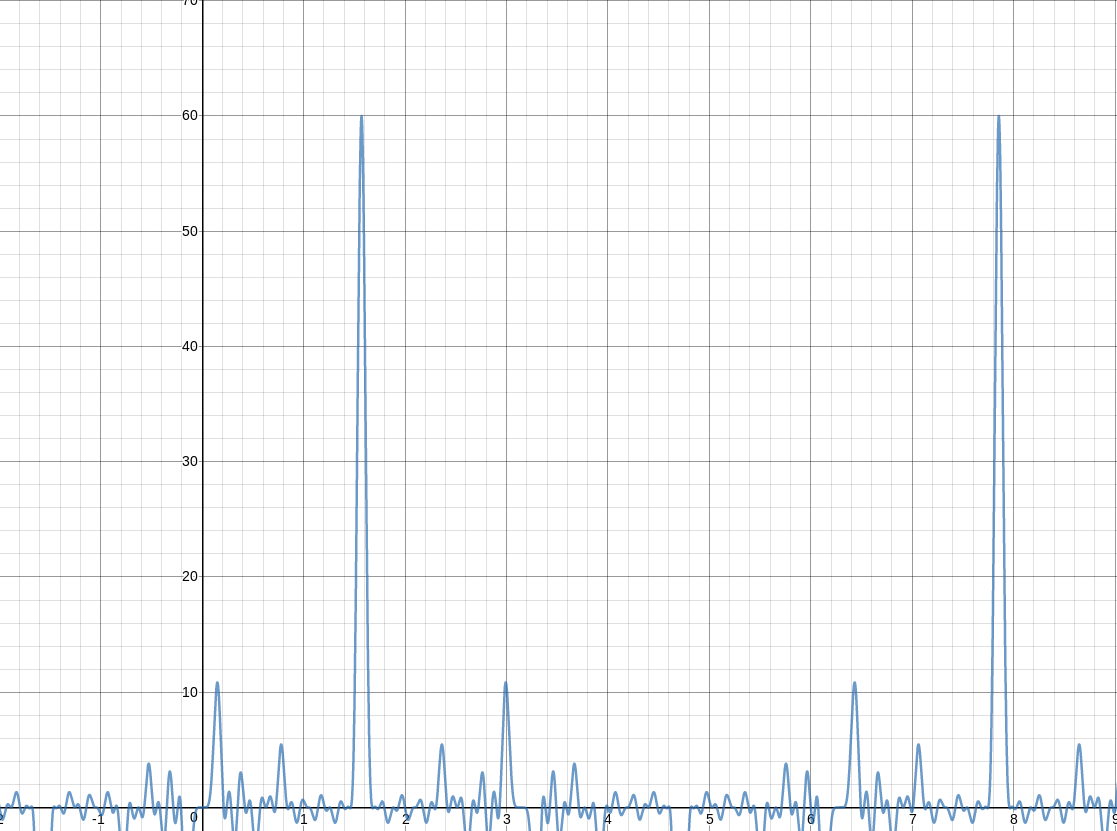
\includegraphics{graph}
    \caption{Gráfico do MMQ}
    \label{fig:graphMMQ}
\end{figure}